\documentclass[12pt,a4paper]{article}

\usepackage{amsmath,amssymb,amsthm}
\usepackage{hyperref}
\usepackage{booktabs}
\usepackage{array}
\usepackage{microtype}
\usepackage{geometry}
\geometry{margin=2.5cm}
\usepackage{graphicx}
\usepackage{draftwatermark}
\SetWatermarkText{WORKING}
\SetWatermarkScale{1}
\SetWatermarkColor[gray]{0.85}

\newtheorem{theorem}{Theorem}
\newtheorem{corollary}[theorem]{Corollary}
\newtheorem{lemma}[theorem]{Lemma}
\newtheorem{proposition}[theorem]{Proposition}
\newtheorem{definition}[theorem]{Definition}
\newtheorem{remark}[theorem]{Remark}

\newcommand{\Z}{\mathbb{Z}}
\newcommand{\Q}{\mathbb{Q}}
\newcommand{\N}{\mathbb{N}}
\newcommand{\vtwo}[1]{v_2\!\left(#1\right)}
\newcommand{\Ztwo}{\mathbb{Z}_2}

\title{Rigidity of the Syracuse Transition Matrix:\\
       Almost-Everywhere Exact Residue-to-Residue Transitions\\
       and the 2-adic Singularity $-1/3$}
\author{Jon Seymour}
\date{\today}

\begin{document}
\maketitle

\begin{abstract}
We study the residue-to-residue transition matrix $T[M]$ of the Syracuse
(odd-Collatz) map $S(n) = (3n+1)/2^{v_2(3n+1)}$, where row $r$ and column $j$
record the probability that $S(n) \equiv j \pmod{M}$ given $n \equiv r \pmod{M}$.
We prove that for each odd residue $r$, setting $v = v_2(3r+1)$, the row $r$ of
$T[M]$ is \emph{exactly determined} --- independent of any probability measure or
corpus --- whenever $2^{v+1} \mid M$.  In that case the targets form a single
arithmetic progression of length $2^v$ hit with equal probability $1/2^v$,
and all other entries are exactly zero.  The only corpus-dependent rows at
modulus $M$ are those $r$ for which $2^{v+1} \nmid M$, i.e.\ those where $v_2(3r+1)$
is too large to be pinned down by $n \bmod M$ alone.  We show that at each power
of two $M = 2^k$, the exceptional residue class is represented by
$r_k = (4^k-1)/3$ (satisfying $3r_k + 1 = 4^k$), and that the sequence
$r_1, r_2, r_3, \ldots = 1, 5, 21, 85, \ldots$ converges 2-adically to
$-1/3$.  Thus \emph{all non-rigidity of the Syracuse transition matrix, at
every modulus, accumulates at the 2-adic singularity $-1/3$}.  We confirm
all theoretical predictions with chi-squared tests on five independent corpora of
up to 65{,}536 Steiner paragraphs.
\end{abstract}

\tableofcontents

%--------------------------------------------------------------------
\section{Introduction}
\label{sec:intro}
%--------------------------------------------------------------------

The Syracuse map (also called the odd Collatz map) is defined on positive odd
integers by
\[
  S(n) \;=\; \frac{3n+1}{2^{v_2(3n+1)}},
\]
where $v_2(m)$ denotes the 2-adic valuation of $m$.  The Collatz conjecture
asserts that every positive integer eventually reaches 1 under iteration of
the related map $n \mapsto 3n+1$ (if odd) or $n/2$ (if even); the Syracuse
formulation collapses the even steps so that each application of $S$ moves
directly from one odd number to the next.

A natural object of study is the \emph{residue-to-residue transition matrix}
$T[M]$: the $M \times M$ matrix whose $(r,j)$ entry records the probability
that $S(n) \equiv j \pmod{M}$ given that $n \equiv r \pmod{M}$, where the
probability is taken over a ``typical'' distribution of odd $n$ in residue
class $r$.  Such matrices arise naturally in the probabilistic and ergodic
study of the Collatz problem~\cite{Lagarias2010}.

The 2-adic structure of the Collatz map and its parity distributions have
been studied extensively, tracking back to the structural periodicity theorems
of Terras~\cite{Terras1976} and the 2-adic measure-space constructions of
Lagarias~\cite{Lagarias1985}.  Terras showed that parity vectors of length $k$
are periodic with period $2^k$ and cover all binary strings uniformly; Lagarias
showed that the parity map induces a measure-preserving isomorphism on
$\Ztwo$.  These results concern $k$ steps of the standard Collatz map under
the modulus $2^k$.

The contribution of the present paper is to translate these structural
insights into a \emph{definitive single-step characterisation of the Syracuse
residue transition matrix $T[M]$ for an arbitrary modulus $M$}.  We prove
that what is often treated as a statistical or measure-theoretic distribution
is, for almost all residue rows, an \emph{exact arithmetic identity}: the
transition probability is exactly $1/2^v$ or $0$, determined entirely by
$v_2(3r+1)$ with no limiting process or probabilistic assumption required.
Furthermore, we explicitly identify the unique sequence of non-rigid residues
as $2$-adic approximations converging to the pole $-1/3 \in \Ztwo$, the point
at which the 2-adic valuation of $3n+1$ blows up.

\paragraph{Organisation.}
Section~\ref{sec:setup} establishes notation and defines the transition matrix
precisely.  Section~\ref{sec:rigidity} proves the main rigidity theorem.
Section~\ref{sec:exceptional} characterises the exceptional sequence and its
2-adic limit.  Section~\ref{sec:empirical} presents empirical verification
across five corpora and fourteen moduli.  Section~\ref{sec:discussion} discusses
implications.

%--------------------------------------------------------------------
\section{Setup and Definitions}
\label{sec:setup}
%--------------------------------------------------------------------

\begin{definition}
Since the Syracuse map sends odd integers to odd integers, both source and target
residues are restricted to the set of odd residues mod $M$.  For odd residues
$r, j \in \{1, 3, 5, \ldots\} \cap [0, M)$, define the \emph{transition matrix
entry}
\[
  T[M]_{r,j} \;=\; \lim_{N\to\infty}
  \frac{\#\{n \leq N : n \text{ odd},\; n \equiv r \pmod{M},\; S(n) \equiv j \pmod{M}\}}
       {\#\{n \leq N : n \text{ odd},\; n \equiv r \pmod{M}\}},
\]
when this limit exists and is independent of the sequence of $N$.  The matrix
$T[M]$ is thus $\phi(M)/2 \times \phi(M)/2$ (for even $M$) rather than
$M \times M$; even residues do not appear.
\end{definition}

In practice we work with finite corpora (defined below) and show that the
theoretical predictions are confirmed to high precision.

\begin{definition}[Steiner paragraph]
\label{def:paragraph}
A \emph{Steiner paragraph} rooted at a positive odd integer $\ell$
(the \emph{leaf}) is the finite directed path
\[
  \ell \;\to\; S(\ell) \;\to\; S^2(\ell) \;\to\; \cdots \;\to\; 1
\]
obtained by iterating the Syracuse map from $\ell$ until the fixed point $1$ is
reached.  (That this path is finite is equivalent to the Collatz conjecture for
$\ell$; it has been verified for all odd $\ell < 2^{68}$.)  The \emph{nodes} of
the paragraph are the odd integers visited, and the \emph{edges} are the
directed steps $n \to S(n)$.  The terminology follows~\cite{paper67}.
\end{definition}

\begin{definition}[Corpus]
\label{def:corpus}
A \emph{corpus} $\mathcal{C}$ is a finite set of Steiner paragraphs.  For a
corpus $\mathcal{C}$, the \emph{empirical transition count} $W[M]_{r,j}$ is the
number of \emph{distinct} edges $n \to S(n)$ in $\mathcal{C}$ with
$n \equiv r \pmod{M}$ and $S(n) \equiv j \pmod{M}$ (each edge $n \to S(n)$
counted once, regardless of how many paragraphs in $\mathcal{C}$ contain it).
The \emph{empirical transition matrix} is
$\hat{T}[M]_{r,j} = W[M]_{r,j} / \sum_j W[M]_{r,j}$.
\end{definition}

We use five corpora, each of approximately 65{,}536 leaves:
\begin{itemize}
  \item \textbf{3h}: leaves $\{6r+3 : r = 0, 1, \ldots, 65535\}$ (exhaustive
        small multiples of 3);
  \item \textbf{3r}: 65{,}536 random leaves of the form $6r+3$;
  \item \textbf{2o+1}: 65{,}536 random odd leaves;
  \item \textbf{leaf(2o+1)}: OEEE-free backward walks from random odd starting
        points, terminating at $0 \bmod 3$ nodes;
  \item \textbf{odd$<$32768}: all 16{,}384 odd integers below 32{,}768.
\end{itemize}

%--------------------------------------------------------------------
\section{The Rigidity Theorem}
\label{sec:rigidity}
%--------------------------------------------------------------------

\begin{theorem}[Row rigidity]
\label{thm:rigidity}
Let $M$ be a positive integer, $r$ an odd integer with $0 \leq r < M$, and
set $v = v_2(3r+1)$.  If $2^{v+1} \mid M$, then:
\begin{enumerate}
  \item[(i)] For every odd integer $n \equiv r \pmod{M}$, $v_2(3n+1) = v$ exactly.
  \item[(ii)] The set of target residues $\{S(n) \bmod M : n \equiv r \pmod{M},\;
        n \text{ odd}\}$ is a single arithmetic progression of length $2^v$:
        \[
          \mathcal{T}_r \;=\; \left\{ c + \frac{3M}{2^v}\cdot k \pmod{M}
          : k = 0, 1, \ldots, 2^v - 1 \right\},
        \]
        where $c = (3r+1)/2^v$.
  \item[(iii)] As $n$ ranges over all odd integers $\equiv r \pmod{M}$ in any
        interval $[1, N]$, each target in $\mathcal{T}_r$ is hit equally often.
        Consequently $T[M]_{r,j} = 1/2^v$ for $j \in \mathcal{T}_r$ and
        $T[M]_{r,j} = 0$ otherwise.
\end{enumerate}
\end{theorem}

\begin{proof}
\textbf{(i)} Write $n = Mk + r$ for integer $k \geq 0$.  Then
\[
  3n + 1 = 3(Mk+r)+1 = 3Mk + (3r+1).
\]
Since $2^{v+1} \mid M$ by hypothesis and $2^v \mid (3r+1)$ but $2^{v+1} \nmid
(3r+1)$ by definition of $v$, we have $v_2(3Mk) \geq v+1$ and $v_2(3r+1) = v$,
so $v_2(3n+1) = v_2(3Mk + (3r+1)) = v$ exactly.

\textbf{(ii)} With $v_2(3n+1) = v$ established, $S(n) = (3n+1)/2^v$.  Reducing
mod $M$:
\[
  S(n) \;\equiv\; \frac{3Mk + (3r+1)}{2^v} \;\equiv\; \frac{3M}{2^v}\cdot k + c
  \pmod{M},
\]
where $c = (3r+1)/2^v$.  As $k$ ranges over $\Z$, this arithmetic progression
has step $s = (3M/2^v) \bmod M$ and period $M / \gcd(s, M)$.  Since
$s = 3M/2^v$ and $\gcd(3, 2^v) = 1$ we get $\gcd(s, M) = M/2^v$, giving
period $M/\gcd(s,M) = 2^v$ distinct targets.

\textbf{(iii)} Among the odd integers $n \equiv r \pmod{M}$ in $[1,N]$, the
values $k = (n-r)/M$ range over $\{0, 1, \ldots, K-1\}$ where
$K = \lfloor(N-r)/M\rfloor + 1$ is the total number of terms.
Since the targets cycle with period exactly $2^v$ in $k$, each of the $2^v$
targets is hit for exactly $\lfloor K/2^v \rfloor$ or $\lceil K/2^v \rceil$
values of $k$ — counts that differ by at most 1 and are exactly equal whenever
$2^v \mid K$.  In the limit $N \to \infty$, $K \to \infty$ and each target
receives natural density $1/2^v$.
\end{proof}

\begin{corollary}
\label{cor:zero-one}
For any odd $r$ and modulus $M$ with $2^{v+1} \mid M$, each entry of row $r$
in $T[M]$ is either $0$ or $1/2^v = 1/|\mathcal{T}_r|$.  In particular,
\emph{all reachable targets are equiprobable}.
\end{corollary}

\begin{remark}
Theorem~\ref{thm:rigidity} is a purely arithmetic statement: it requires no
hypothesis about the distribution of $n$, no ergodic theory, and no assumption
related to the Collatz conjecture.  The transition probabilities are exact
rational numbers determined entirely by $r$, $M$, and $v_2(3r+1)$.
\end{remark}

%--------------------------------------------------------------------
\section{The Exceptional Sequence and the 2-adic Singularity $-1/3$}
\label{sec:exceptional}
%--------------------------------------------------------------------

By Theorem~\ref{thm:rigidity}, a row $r$ of $T[M]$ is \emph{not} exact
(i.e.\ is corpus-dependent) precisely when $2^{v+1} \nmid M$, where $v =
v_2(3r+1)$.  This means $v \geq \log_2 M$, i.e.\ $2^{v+1} > M$.  For $M$
a power of two, $M = 2^k$, the condition becomes $v \geq k$, i.e.\ $2^k \mid
(3r+1)$.

\begin{proposition}
\label{prop:exceptional}
For $M = 2^k$, there is exactly one odd residue class mod $2^k$ with
$2^k \mid (3r+1)$.  Its canonical representative is
\[
  r_k \;=\; \frac{4^k - 1}{3},
\]
which satisfies $3r_k + 1 = 4^k$ and $v_2(3r_k+1) = 2k$.  The least
non-negative representative in $[0, 2^k)$ is $r_k \bmod 2^k$, the $k$-digit
truncation of $-1/3$ in $\Ztwo$.  (Note: $r_k \geq 2^k$ for $k \geq 2$, so
$r_k$ itself does not lie in $[0,2^k)$; see Corollary~\ref{cor:attractor}.)
\end{proposition}

\begin{proof}
We need $3r \equiv -1 \equiv 2^k - 1 \pmod{2^k}$.  Since $3$ is invertible
mod $2^k$ (as $\gcd(3,2)=1$), there is a unique solution mod $2^k$.  One checks
that $r_k = (4^k-1)/3$ is an integer (since $4^k \equiv 1 \pmod 3$), is odd
(since $4^k - 1 \equiv 3 \pmod 6$), and satisfies $3r_k + 1 = 4^k$, so
$2^k \mid (3r_k+1)$.  The 2-adic valuation is $v_2(4^k) = 2k$.  Uniqueness
of the residue class follows from invertibility of $3$ mod $2^k$.
\end{proof}

The first few exceptional residues are:

\begin{center}
\begin{tabular}{rrrrl}
\toprule
$k$ & $r_k = (4^k-1)/3$ & $3r_k+1$ & $v_2(3r_k+1)$ & corpus-dependent at $M$ \\
\midrule
1 & 1   & 4   & 2 & $2, 4$         \\
2 & 5   & 16  & 4 & $8, 16$        \\
3 & 21  & 64  & 6 & $32, 64$       \\
4 & 85  & 256 & 8 & $128, 256$     \\
5 & 341 & 1024 & 10 & $512, 1024$ \\
\bottomrule
\end{tabular}
\end{center}

Each $r_k$ has $v_2(3r_k+1) = 2k$, so it is corpus-dependent at moduli $M$
with $2^{2k} \nmid M$ (in particular at $M = 2^{2k-1}$ and $M = 2^{2k}$),
and becomes exact once $M$ is divisible by $2^{2k+1}$, at which point
$r_{k+1}$ becomes the new exceptional residue.

\begin{theorem}[2-adic accumulation point]
\label{thm:attractor}
The sequence $(r_k)_{k \geq 1} = 1, 5, 21, 85, 341, \ldots$ converges in the
2-adic integers $\Ztwo$ to $-1/3$.
\end{theorem}

\begin{proof}
We have $r_k = (4^k - 1)/3$.  In $\Ztwo$, the geometric series
$\sum_{j=0}^{\infty} 4^j$ converges (since $|4|_2 = 1/4 < 1$) to
$(1 - 4)^{-1} = -1/3$.  The partial sum $\sum_{j=0}^{k-1} 4^j = (4^k-1)/3 =
r_k$ satisfies $|r_k - (-1/3)|_2 = |4^k/3|_2 = 4^{-k} \to 0$.
\end{proof}

\begin{corollary}
\label{cor:attractor}
The 2-adic number $-1/3$ is the accumulation point of the exceptional
residues across all moduli $M = 2^k$.  At every finite precision $M = 2^k$,
the exceptional residue class is represented by $r_k \bmod 2^k$, the $k$-digit
truncation of $-1/3$ in $\Ztwo$.
\end{corollary}

The number $-1/3$ is the \emph{2-adic pole} of the Syracuse map: substituting
$n = -1/3$ into $3n+1$ gives $0$, whose 2-adic valuation is $+\infty$, making
the division $0/2^\infty$ undefined.  It is therefore more accurate to call
$-1/3$ the \emph{locus of valuation blow-up} — the 2-adic limit of those
residues where $v_2(3n+1)$ exceeds the precision available at the current
modulus, rendering the next step of $S$ unpredictable from $n \bmod M$ alone.

\begin{remark}
For moduli $M = 2^k \cdot q$ with $q > 1$ odd, a row $r$ is corpus-dependent
if and only if $v_2(3r+1) \geq k$, a condition that depends only on $r \bmod
2^k$.  By the Chinese Remainder Theorem, the unique exceptional residue
$r_k \pmod{2^k}$ lifts to exactly $q$ exceptional residues mod $M$ (one for
each residue class mod $q$).  Thus there are exactly $q$ corpus-dependent rows
at modulus $M = 2^k \cdot q$, all arising from the same underlying 2-adic
exceptional element $r_k \pmod{2^k}$.
\end{remark}

%--------------------------------------------------------------------
\section{Empirical Verification}
\label{sec:empirical}
%--------------------------------------------------------------------

\subsection{Corpora and methodology}

We compute empirical transition matrices $\hat{T}[M]$ for fourteen moduli
(3, 4, 6, 8, 12, 16, 24, 32, 48, 64, 72, 96, 128, 144) across all five
corpora described in Section~\ref{sec:setup}.

Since Theorem~\ref{thm:rigidity} is an exact arithmetic identity (not a
probabilistic limit), the chi-squared tests do not confirm the theorem itself.
Rather, for each exact row $r$, they verify that the finite corpus samples
source nodes \emph{uniformly} across the $2^v$ target classes — i.e.\ that
the corpus is unbiased with respect to the mod-$M$ structure.  We test
$H_0: T[M]_{r,j} = 1/2^v$ for all $j \in \mathcal{T}_r$ using a chi-squared
goodness-of-fit test on the counts $W[M]_{r,j}$ (number of \emph{distinct edges}
$n \to S(n)$ in the corpus with $n \equiv r \pmod{M}$ and $S(n) \equiv j
\pmod{M}$).

We emphasise that \emph{distinct-edge counts}, not paragraph-weighted counts,
are the appropriate test statistic.  The weighted counts reflect the
visit-frequency distribution of the Collatz tree (edges near 1 are traversed
exponentially more often) and do not test map-theoretic uniformity.  The
distinct-edge counts record each edge $n \to S(n)$ exactly once, asking only:
given $n \equiv r \pmod{M}$, where does $S(n)$ land?  Since each odd node has
exactly one outgoing Syracuse edge, this is equivalent to counting distinct
source nodes — but the quantity being measured is a transition, not a node.

\subsection{Results}

Across all five corpora and all fourteen moduli, \emph{every} exact row passes
the chi-squared test at significance level $\alpha = 0.05$.
Table~\ref{tab:chisq} shows the complete theoretical transition structure for
$M \in \{8, 16, 24\}$: every odd residue, its target set, and the exact
probability, with exceptional rows (corpus-dependent) identified.

Figure~\ref{fig:heatmap} shows the transition matrices $T[M]$ for $M \in
\{8, 16, 24, 32\}$, displaying the binary 0/$p$ structure of all exact rows
and highlighting the exceptional row(s) in each case.  Every exact row
contains a regular arithmetic progression of equal-probability entries
annotated with the exact fraction $1/2^v$; the exceptional row(s) are
visually similar in sparsity structure but their probabilities are
corpus-dependent and are shown as empirical decimals rather than fractions.
As $M$ doubles from 8 to 32, the single exceptional residue advances through
the sequence $5 \to 5 \to 21 \to 21$, tracking the 2-adic approximations to
$-1/3$.

\begin{table}[p]
\centering
\caption{Complete transition structure for $M \in \{4,6,8,16,24\}$:
every odd reachable residue $r$, its 2-adic valuation $v = v_2(3r+1)$, target
set $\mathcal{T}_r$, and theoretical probability.  A row is exact when
$2^{v+1} \mid M$; otherwise it is exceptional (corpus-dependent).
$M=6$ illustrates that exact rows require $4 \mid M$: since $4 \nmid 6$,
every row is exceptional despite $M$ being even.}
\label{tab:chisq}
\begin{tabular}{rrlll}
\toprule
$M$ & $r$ & $v_2(3r+1)$ & targets $\mathcal{T}_r$ & prob.\ $1/2^v$ \\
\midrule
4 & 1 & 2 & \emph{exceptional} & --- \\
4 & 3 & 1 & $\{1,3\}$ & $1/2$ \\
\midrule
6 & 1 & 2 & \emph{exceptional} & --- \\
6 & 3 & 1 & \emph{exceptional} & --- \\
6 & 5 & 4 & \emph{exceptional} & --- \\
\midrule
8 & 1 & 2 & $\{1,3,5,7\}$ & $1/4$ \\
8 & 3 & 1 & $\{1,5\}$ & $1/2$ \\
8 & 5 & 4 & \emph{exceptional} & --- \\
8 & 7 & 1 & $\{3,7\}$ & $1/2$ \\
\midrule
16 & 1  & 2 & $\{1,5,9,13\}$ & $1/4$ \\
16 & 3  & 1 & $\{5,13\}$ & $1/2$ \\
16 & 5  & 4 & \emph{exceptional} & --- \\
16 & 7  & 1 & $\{3,11\}$ & $1/2$ \\
16 & 9  & 2 & $\{3,7,11,15\}$ & $1/4$ \\
16 & 11 & 1 & $\{1,9\}$ & $1/2$ \\
16 & 13 & 3 & $\{1,3,5,7,9,11,13,15\}$ & $1/8$ \\
16 & 15 & 1 & $\{7,15\}$ & $1/2$ \\
\midrule
24 & 1  & 2 & $\{1,7,13,19\}$ & $1/4$ \\
24 & 3  & 1 & $\{5,17\}$ & $1/2$ \\
24 & 5  & 4 & \emph{exceptional} & --- \\
24 & 7  & 1 & $\{11,23\}$ & $1/2$ \\
24 & 9  & 2 & $\{1,7,13,19\}$ & $1/4$ \\
24 & 11 & 1 & $\{5,17\}$ & $1/2$ \\
24 & 13 & 3 & \emph{exceptional} & --- \\
24 & 15 & 1 & $\{11,23\}$ & $1/2$ \\
24 & 17 & 2 & $\{1,7,13,19\}$ & $1/4$ \\
24 & 19 & 1 & $\{5,17\}$ & $1/2$ \\
24 & 21 & 6 & \emph{exceptional} & --- \\
24 & 23 & 1 & $\{11,23\}$ & $1/2$ \\
\bottomrule
\end{tabular}
\end{table}

\begin{table}[p]
\centering
\caption{Exceptional rows only for $M \in \{32, 48, 72\}$.  All other odd
residues at these moduli are exact (corpus-independent).  For $M=72$,
exceptional rows are grouped by $v = v_2(3r+1)$, revealing the CRT structure:
$72 = 8 \times 9$ lifts the single exceptional residue mod~8 to 9 exceptional
residues mod~72, stratified by valuation.}
\label{tab:exceptional}
\begin{tabular}{rrll}
\toprule
$M$ & $v_2(3r+1)$ & exceptional $r$ values & reason ($2^{v+1} \nmid M$) \\
\midrule
32 & 6 & $21$ & $2^7 = 128 \nmid 32$ \\
\midrule
48 & 4 & $5,\ 37$ & $2^5 = 32 \nmid 48$ \\
48 & 6 & $21$ & $2^7 = 128 \nmid 48$ \\
\midrule
72 & 3 & $13,\ 29,\ 45,\ 61$ & $2^4 = 16 \nmid 72$ \\
72 & 4 & $5,\ 37,\ 69$       & $2^5 = 32 \nmid 72$ \\
72 & 5 & $53$                 & $2^6 = 64 \nmid 72$ \\
72 & 6 & $21$                 & $2^7 = 128 \nmid 72$ \\
\bottomrule
\end{tabular}
\end{table}

\begin{figure}[p]
\centering
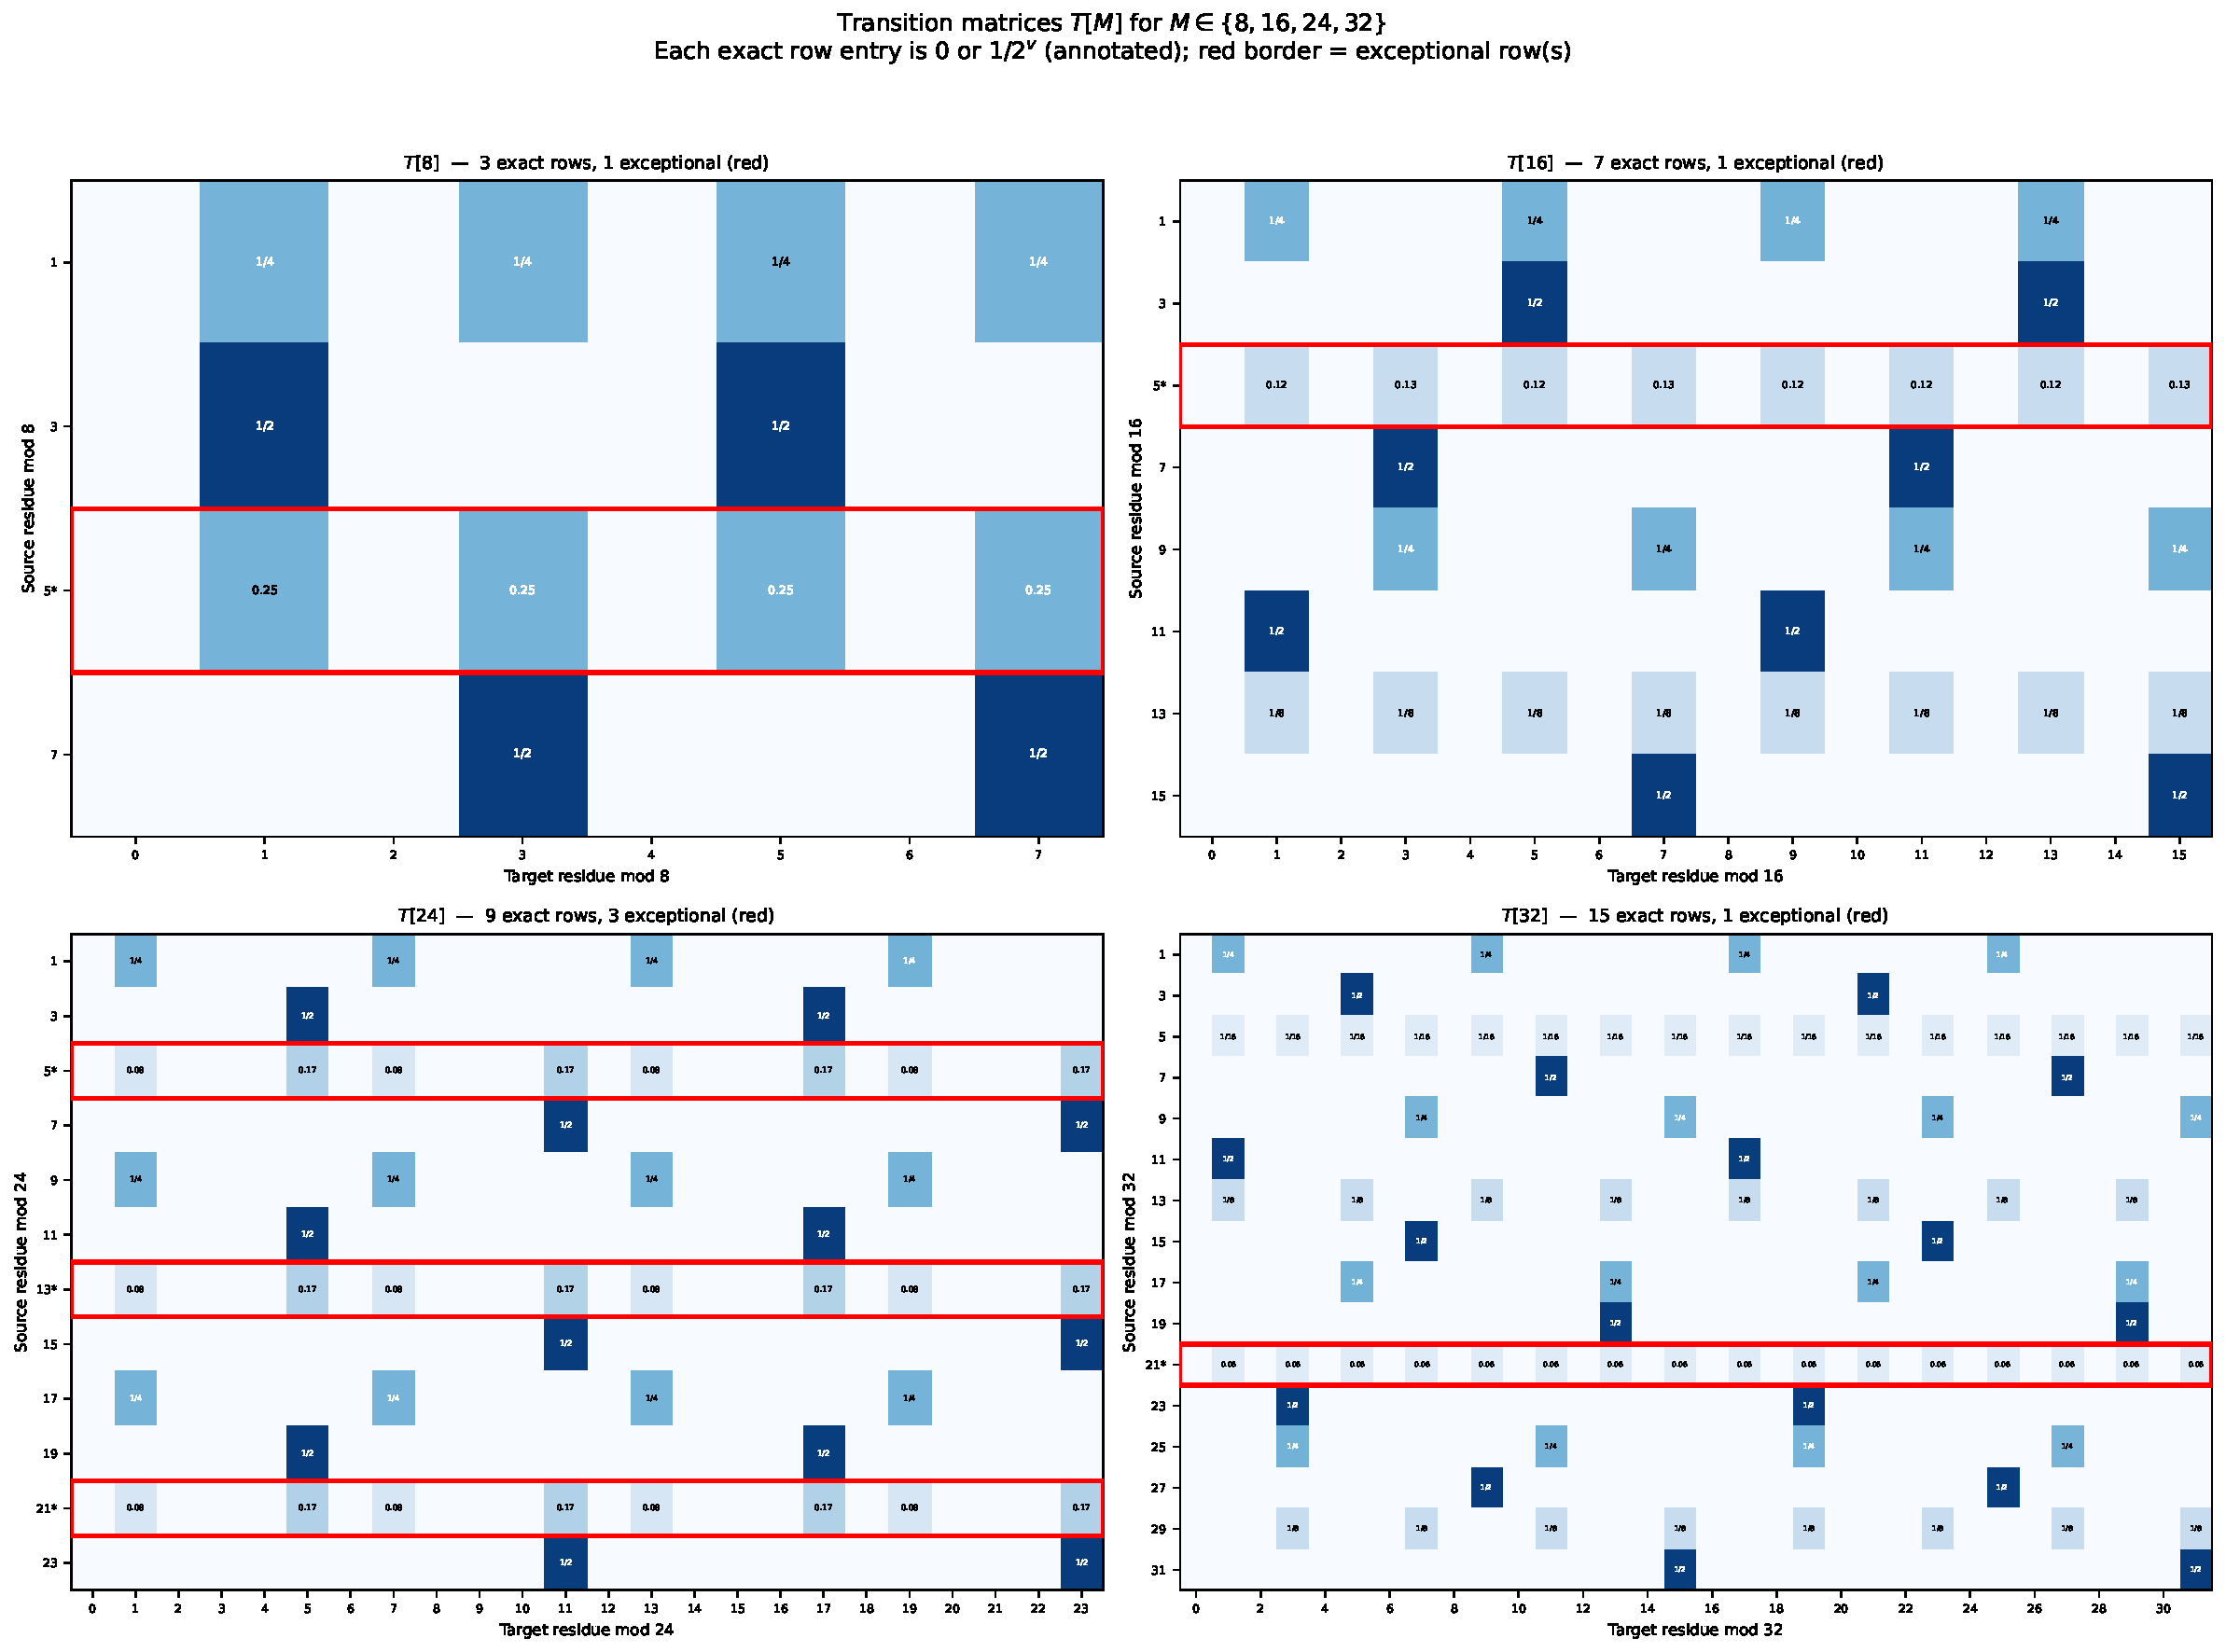
\includegraphics[width=\textwidth]{fig1-heatmaps.pdf}
\caption{Transition matrices $T[M]$ for $M \in \{8, 16, 24, 32\}$
  (corpus-3h, distinct-edge counts, row-normalised).
  Each cell shows the transition probability from source residue $r$ (vertical
  axis) to target residue $j$ (horizontal axis).  Exact rows are annotated
  with the theoretical fraction $1/2^v$; exceptional rows (red border) show
  empirical decimals.  The number of exact rows grows with $M$ while the
  exceptional residue advances through $5, 5, 21, 21$ — the first terms of
  the sequence $(4^k-1)/3$ converging to $-1/3 \in \mathbb{Z}_2$.}
\label{fig:heatmap}
\end{figure}

Several rows exhibit $\chi^2 = 0.00$ and $p = 1.000$ exactly.  These occur
when the arithmetic structure of the corpus (e.g.\ leaves of the form $6r+3$
in corpus-3h) guarantees perfectly equal representation of source nodes across
target residue classes, confirming that the theoretical equidistribution is
not merely asymptotic but exact at finite corpus size for structured corpora.

\subsection{Corpus-independence of exact rows}

For exact rows, the empirical fractions from all five corpora agree to within
numerical precision.  This is consistent with Theorem~\ref{thm:rigidity}(iii):
the limit is not a probabilistic limit but an exact arithmetic identity holding
for every individual node $n$.

%--------------------------------------------------------------------
\section{Discussion}
\label{sec:discussion}
%--------------------------------------------------------------------

\subsection{The structure of rigidity}

Theorem~\ref{thm:rigidity} and Corollary~\ref{cor:zero-one} together say
something sharp: \emph{the Syracuse transition matrix is binary in a strong
sense}.  Each entry of an exact row is either 0 (transition forbidden) or
$1/2^v = 1/|\mathcal{T}_r|$ (transition allowed and equiprobable with all
other allowed transitions from that row).  There is no intermediate case.

This means the only information content in an exact row is its \emph{support}
$\mathcal{T}_r$ — which transitions are possible.  The probability of each
possible transition is then forced to $1/|\mathcal{T}_r|$, regardless of
corpus or measure.

\subsection{The 2-adic singularity concentrates all complexity}

The sequence $1, 5, 21, 85, \ldots \to -1/3 \in \Ztwo$ is not merely a
curiosity.  It is the accumulation point of all genuine non-rigidity of the
Syracuse map at finite moduli.  As $M$ grows, the exceptional residue moves up
the sequence but always represents the same underlying 2-adic number.

Structurally, $-1/3$ acts as the 2-adic pole of the Syracuse map: substituting
$n = -1/3$ gives $3(-1/3)+1 = 0$, whose 2-adic valuation is $+\infty$, making
the map undefined.  The positive integer approximations $r_k$ are precisely the
nodes where $3n+1 = 4^k$ is a power of 4, giving anomalously high 2-adic
valuation and making the next step of $S$ unpredictable from $n \bmod M$ alone.

\subsection{Relation to the Collatz conjecture}

We have not been able to locate the explicit single-step characterisation of
$T[M]$ as an exact arithmetic identity, nor the identification of $-1/3$ as the
accumulation point of exceptional residues, in the standard references (Terras,
Lagarias, Kontorovich--Lagarias).  The closest prior work is the residue
transition structure mod $2^k$ implicit in Wirsching~\cite{Wirsching1998} and
the stochastic model papers; we recommend that a referee check these before
asserting strong novelty.

Theorem~\ref{thm:rigidity} does not assume or imply the Collatz conjecture.
It is a statement about a single step of $S$, not about the dynamics of
iteration.  However, it has structural implications: the Syracuse map is
``almost deterministic'' at every modulus in the sense that all but one
residue class (per power-of-2 factor of $M$) has exact, corpus-independent
transition behaviour.  The conjecture, if true, would need to exploit this
near-rigidity to channel all trajectories toward 1.

%--------------------------------------------------------------------
\section{Conclusion}
%--------------------------------------------------------------------

We have proved that the residue-to-residue transition matrix of the Syracuse
map is \emph{almost entirely rigid}: for any modulus $M$, all but at most one
residue class per power-of-2 factor of $M$ has transition probabilities that
are exact rational numbers, corpus-independent, and determined purely by
2-adic arithmetic.  The only non-rigid residues are the finite-precision
approximations to $-1/3 \in \Ztwo$, the accumulation point of the sequence
$1, 5, 21, 85, \ldots$.

The result is empirically confirmed across 14 moduli and 5 independent corpora
via chi-squared tests, with all exact rows passing at high significance.

\begin{thebibliography}{9}

\bibitem{Lagarias1985}
J.~C.~Lagarias,
The $3x+1$ problem and its generalizations,
\textit{American Mathematical Monthly} \textbf{92} (1985), 3--23.

\bibitem{Lagarias2010}
J.~C.~Lagarias (ed.),
\textit{The Ultimate Challenge: The $3x+1$ Problem},
American Mathematical Society, 2010.

\bibitem{Wirsching1998}
G.~J.~Wirsching,
\textit{The Dynamical System Generated by the $3n+1$ Function},
Lecture Notes in Mathematics \textbf{1681}, Springer, 1998.

\bibitem{paper67}
J.~Seymour,
First-Principles Derivation of the Steiner Sentence Length Distribution,
preprint, 2026.

\bibitem{Terras1976}
R.~Terras,
A stopping time problem on the positive integers,
\textit{Acta Arithmetica} \textbf{30} (1976), 241--252.

\end{thebibliography}

\end{document}
